\documentclass[10pt,openright,twoside,french]{book}

\usepackage{marvosym}
\input philippe2013
\input philippe2013_activites

\usepackage{docmute}

\pagestyle{empty}

\begin{document}
\renewcommand\MaCouleur{Melon!150}

%___________________________
%===    Page de garde
%------------------------------------------------------

\frontmatter

\titlepage{
\begin{center}
{\Large\bfseries\color{\MaCouleur} Philippe \bsc{De Sousa}}

\vspace*{\stretch{1}}

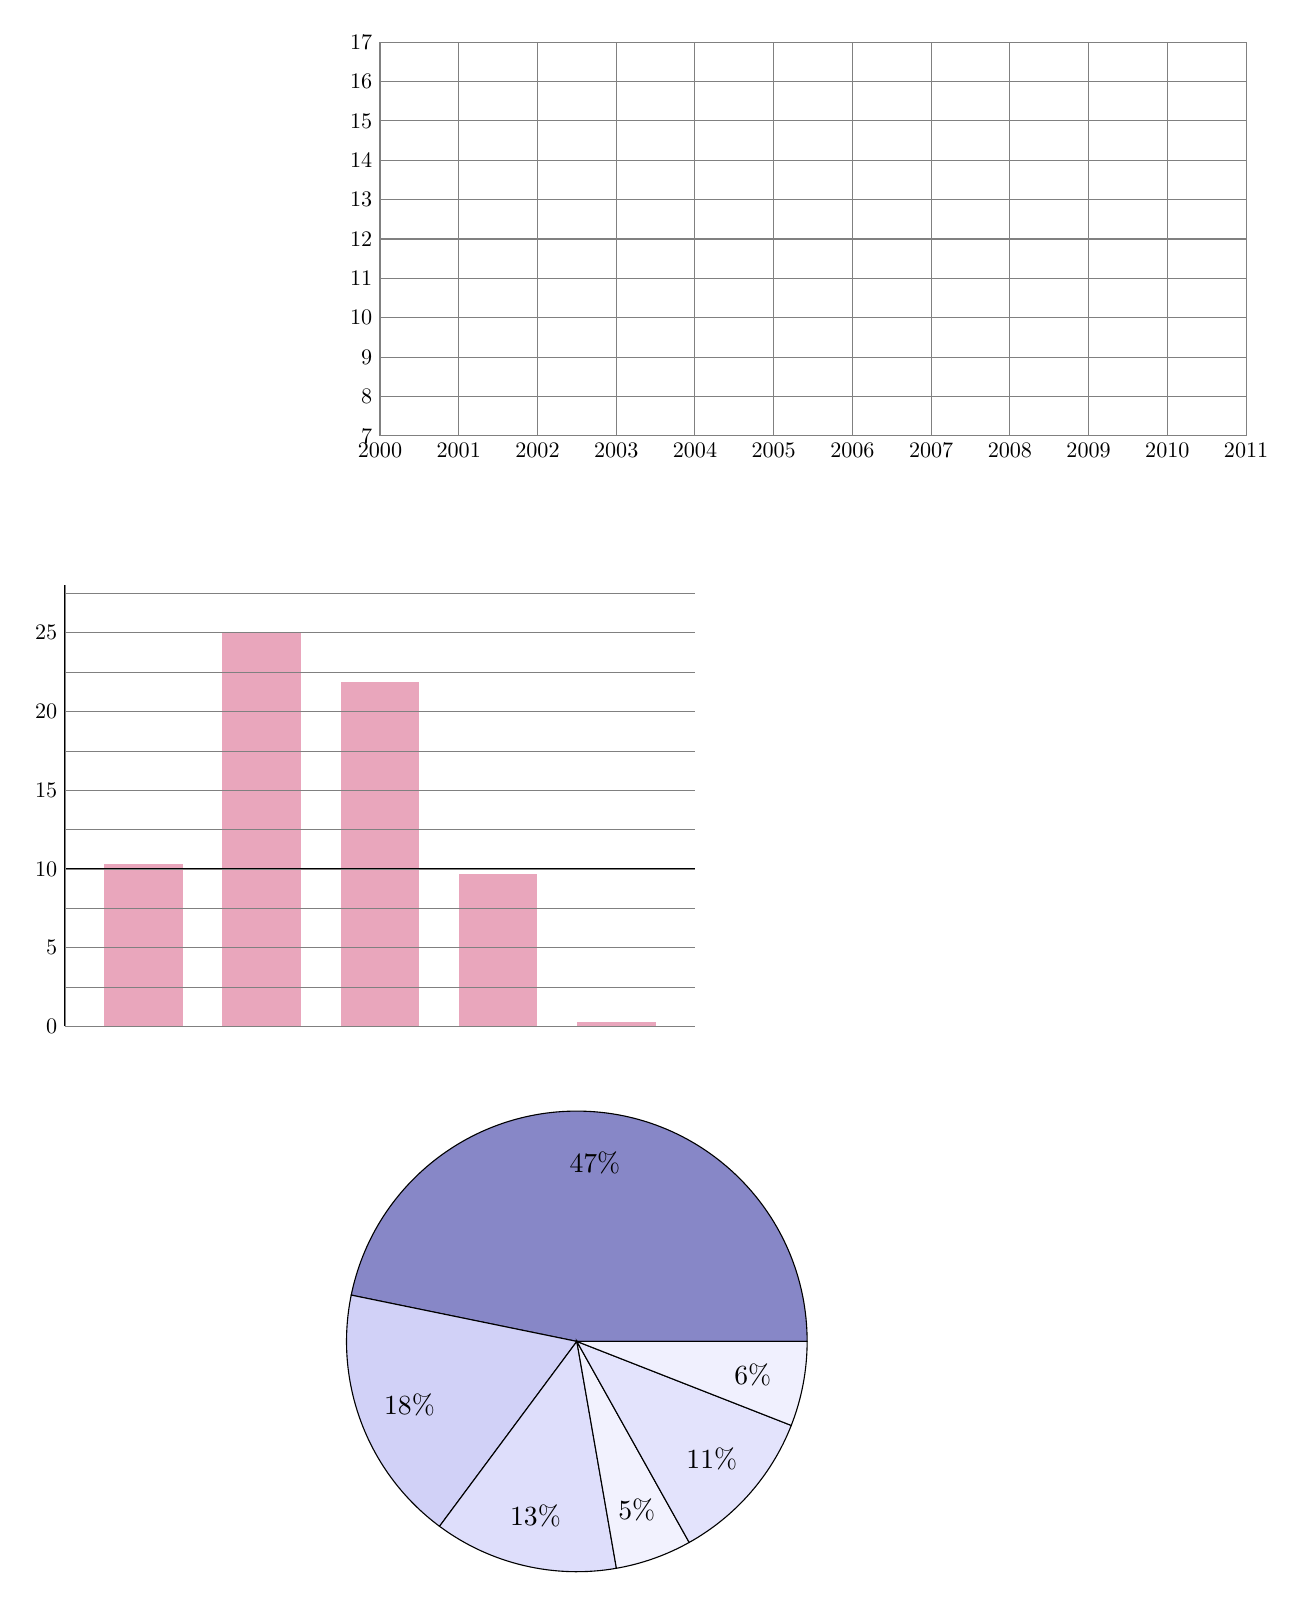
\begin{tikzpicture}
\begin{scope}[xscale=1,yscale=0.2,xshift=-1cm]
\newcommand{\Conso}{(1,10.3)(2.5,25)(4,21.9)(5.5,9.7)(7,0.3)}
\draw[line width=10mm,color=purple!35] plot[ycomb] coordinates {\Conso};
\draw (0,0) grid[xstep=9,ystep=5] (8,28);
\draw[gray,very thin] (0,0) grid[xstep=9,ystep=2.5] (8,28);
\foreach \y in {0,5,...,25} \draw (0,\y) node[left,scale=0.8]{\y};
\end{scope}

\begin{scope}[xshift=3cm,yshift=4cm,yscale=0.5]
\draw[color=OliveGreen,line width=1.5pt] plot[mark=triangle,mark size=3pt] file {Titre1.txt};
\draw[color=blue,line width=1.5pt] plot[mark=diamond,mark size=3pt] file {Titre2.txt};
\draw[thin,gray] (0,7) grid (11,17);
\foreach \y in {7,8,...,17} \draw (0,\y) node[left,scale=0.8]{\y};
\foreach \x in {2000,2001,...,2011} \draw (\x-2000,7) node [below,scale=0.8] {\x};
\end{scope}

\begin{scope}[xshift=5.5cm,yshift=-4cm,scale=0.65]
%\draw[fill=black!47!blue!47] (0,0)--(0:4.5)arc(0:168.4:4.5)--cycle;
%\draw (84:4) node {47\%};
%\draw (84:5.6) node {\bsc{tva}};
\foreach \a/\b/\p/\c in
{
0/168.4/47/\bsc{tva},
168.4/233.4/18/Revenus,
233.4/279.9/13/Sociétés,
279.9/299.2/5/\bsc{tipp},
299.2/338.6/11/{\scriptsize Recettes fiscales},
338.6/360/6/{\scriptsize Recettes}
}{
\draw[fill=black!\p!blue!\p]
(0,0) -- (\a:4.5) arc (\a:\b:4.5) -- cycle;
\draw ({(\a+\b)/2}:3.5) node {\p\%};
}
\end{scope}
\end{tikzpicture}

\begin{tikzpicture}[remember picture,overlay]
\begin{scope}
\node [rotate=45,scale=8,text opacity=0.2]
at (current page.center) {\color{\MaCouleur}\scshape Mathématiques};
\end{scope}
\begin{scope}[xshift=5.5cm,yshift=8cm]
\draw[color=\MaCouleur] (0,0) node[scale=8] {\premiere};
\draw[color=\MaCouleur] (-0.2,-0.15) node[below,scale=6] {\stmg};
\node [below=7cm,scale=4,color=\MaCouleur] at (-0.2,-0.15) {Activités};
\end{scope}
\end{tikzpicture}

\vspace*{\stretch{1}}

D'après le programme $\NP{2012}$
\end{center}
} 

\pieddepage{}{}{}
\entete{}{}{}

\mainmatter

\entete{}{{\color{\MaCouleur} \textbullet~\leftmark~\textbullet}}{}
\pieddepage{}{\color{\MaCouleur}$\stackrel{***}{\thepage}$}{}

%------ Chapitre 01 - Evolutions
    %------------------ Activité 1
        \documentclass[10pt,openright,twoside,french]{book}
\input philippe2013
\input philippe2013_activites
\pagestyle{empty}

\begin{document}

\TitreActivite{i.1}{Calculer une évolution}

\begin{enumerate}
    \item Paul a acheté une veste en solde. Il a payé \EUR{$102$} alors que l'ancien prix était de \EUR{$120$}.\par On note $p_1$ le prix avant les soldes et $p_2$ le prix après les soldes.
        \begin{enumerate}
            \item Le prix de la veste a-t-il augmenté ou diminué ? de combien ?
            \item Recopier et compléter la phrase suivante : {\cursive L'évolution de $p_1$ à $p_2$ est égale à : \ldots}
            \item Calculer, en pourcentage, l'évolution du prix de la veste.
            \item Recopier et compléter la phrase suivante : {\cursive L'évolution de $p_1$ à $p_2$ est égale à : \ldots} \%.
        \end{enumerate}\medskip
    \item Paulette a acheté un pantalon en solde. Elle a payé \EUR{$32$} alors que l'ancien prix était de \EUR{$40$}.\par On note $p_3$ le prix avant les soldes et $p_4$ le prix après les soldes.
        \begin{enumerate}
            \item Le prix du pantalon a-t-il augmenté ou diminué ? de combien ?
            \item Recopier et compléter la phrase suivante : {\cursive L'évolution de $p_3$ à $p_4$ est égale à : \ldots}
            \item Calculer, en pourcentage, l'évolution du prix du pantalon.
            \item Recopier et compléter la phrase suivante : {\cursive L'évolution de $p_3$ à $p_4$ est égale à : \ldots} \%.
        \end{enumerate}\medskip
    \item Paul dit à Paulette : \og~J'ai fait une meilleure affaire que toi !~\fg\par Paulette prétend le contraire.
        \begin{enumerate}
            \item Quel est l'argument de Paul ?
            \item Quel est celui de Paulette ?
            \item Qui a raison ?
        \end{enumerate}
    \item Compléter le tableau suivant :

    \begin{center}
    \renewcommand\arraystretch{1.75}
        \begin{tabular}{|c|c|c|c|c|}
            \hline
                \multirow{2}*{$y_1$} & \multirow{2}*{$y_2$} & Hausse ou baisse & \multicolumn{2}{c|}{Variations de $y_1$ à $y_2$}\\
                \cline{4-5}
                & & de $y_1$ à $y_2$ & Absolue & Relative \\
            \hline
                $10$ & $15$ & &  & \\
            \hline
                $0{,}8$ & $0{,}2$ & &  & \\
            \hline
                $50$ & $40$ & &  & \\
            \hline
                $65$ & $65$ & &  & \\
            \hline
                $0$ & $15$ & & & \\
            \hline
                $150$ & & & $12$ &  \\
            \hline
                & $196$ & & $-4$ & \\
            \hline
                $18$ & & & & $6\%$ \\
             \hline
                $150$ & & & & $-12{,}5\%$ \\
            \hline
        \end{tabular}
    \end{center}
\end{enumerate}

\end{document} \clearpage
    %------------------ Activité 2
        \documentclass[10pt,openright,twoside,french]{book}
\input philippe2013
\input philippe2013_activites
\pagestyle{empty}

\begin{document}

\TitreActivite{i.2}{C{\oe}fficient multiplicateur}

Une petite entreprise emploie deux commerciaux, M. \bsc{Machin} et Mme \bsc{Bidule}.\par
On note $y_1$ le nombre de contrats conclus l'année passée et $y_2$ le nombre de contrats conclus cette année.\medskip

\begin{enumerate}
    \item Le nombre de contrats conclus par M. \bsc{Machin} était l'an dernier de $75$. Il annonce à son patron qu'il a multiplié par $1{,}48$ cette année le nombre de ses contrats signés.
        \begin{enumerate}
            \item Calculer, en utilisant les notations $y_1$ et $y_2$, le nombre de contrats signés cette année. Ce nombre a-t-il augmenté ou diminué ?
            \item Vérifier, en utilisant une formule du cours, que le taux d'évolution $t$ du nombre de contrats conclus de l'année passée à cette année est de $48\%$.
            \item Calculer $1+t$. Que remarque-t-on ?
        \end{enumerate}\smallskip
    \item Le nombre de contrats conclus par Mme \bsc{Bidule} était l'année passée de $120$. Elle annonce à son patron qu'elle a multiplié par $0{,}95$ cette année le nombre de contrats signés.
        \begin{enumerate}
            \item Calculer, en utilisant les notations $y_1$ et $y_2$, le nombre de contrats signés cette année. Ce nombre a-t-il augmenté ou diminué ?
            \item Vérifier, en utilisant une formule du cours, que le taux d'évolution $t$ du nombre de contrats conclus de l'année passée à cette année est de $-5\%$.
            \item Calculer $1+t$. Que remarque-t-on ?
        \end{enumerate}\smallskip
    \item Quel lien peut-on faire entre le \coef multiplicateur et l'évolution ?\smallskip
    \item Compléter le tableau suivant :
    
    \begin{center}
        \renewcommand\arraystretch{1.75}
        \begin{tabularx}{0.95\linewidth}{|c|X|X|}
            \hline
                Lorsqu'une grandeur & \multicolumn{2}{c|}{Cette grandeur est multipliée par :}\\
                \cline{2-3}
                varie de : & s'il s'agit d'une hausse & s'il s'agit d'une baisse \\
            \hline
                $12\%$ & $1 + 12\% = 1 + 0{,}12 = 1{,}12$ & $1 - 12\% = 1 - 0{,}12 = 0{,}88$\\
            \hline
                $1\%$ & & \\
            \hline
                $10{,}4\%$ & & \\
            \hline
                $50\%$ & & \\
            \hline
                $73\%$ & & \\
            \hline
                $115{,}25\%$ & & \\
            \hline
                & $1{,}27 =$ & \\
            \hline
                & $1{,}196 =$ & \\
            \hline
                & & $0{,}85 =$ \\
            \hline
                & & $0{,}713 =$\\
            \hline
        \end{tabularx}
    \end{center}
\end{enumerate}

\end{document} \clearpage
    %------------------ Activité 3
        \documentclass[10pt,openright,twoside,french]{book}
\input philippe2013
\input philippe2013_activites
\pagestyle{empty}

\begin{document}

\TitreActivite{i.3}{Taux d'évolution successifs\par Taux réciproque}

\exo En $\NP{2010}$, un paysan a produit $x$ tonnes de blé.\par
En $\NP{2011}$, sa production a diminué de $8\%$.\par
L'année suivante, il est rassuré car la production a augmenté de $10\%$.

\begin{enumerate}
    \item Le paysan est-il capable de donner rapidement l'évolution globale entre $\NP{2010}$ et $\NP{2012}$ ?
    \item Supposons $x = 500$.
        \begin{enumerate}
            \item À combien de tonnes s'élève sa production en $\NP{2011}$ ? en $\NP{2012}$ ?
            \item Quelle est alors, en pourcentage, l'évolution globale entre $\NP{2010}$ et $\NP{2012}$ ?
        \end{enumerate}
    \item Supposons $x = 635$.
        \begin{enumerate}
            \item À combien de tonnes s'élèvent sa production en $\NP{2011}$ ? en $\NP{2012}$ ?
            \item Quelle est alors, en pourcentage, l'évolution globale entre $\NP{2010}$ et $\NP{2012}$ ?
        \end{enumerate}
    \item Peut-on conclure ?
\end{enumerate}\bigskip

\exo Dans un village au bord de mer, la population est de $125$ habitants.
\begin{enumerate}
    \item Au début des vacances d'été, la population augmente pour atteindre un total de $400$ habitants.\par
        Calculer l'évolution absolue ainsi que le taux d'évolution (en pourcentage) correspondant.
    \item À la fin des vacances, le village retrouve sa population d'origine de $125$ habitants.\par
        Calculer l'évolution absolue ainsi que le taux d'évolution (en pourcentage) correspondant.
    \item Quelles remarques peut-on faire ?
\end{enumerate}

\end{document} \clearpage

%------ Chapitre 02 - Suites
    %------------------ Activité 1
        \documentclass[10pt,openright,twoside,french]{book}
\input preambule_2013

\newcommand\TitreActivite[2]{%
    \setcounter{exo}{0}
        \begin{center}
            \psframebox[shadow=true,shadowcolor=gray!75,shadowsize=3pt,%
            framearc=0.3,%
            fillstyle=gradient,gradmidpoint=0.8,gradangle=20,gradbegin=red!60!yellow!40,gradend= white]{%
                \parbox{0.5\linewidth}{%
                    \begin{center}
                        \Large\bfseries
                        \uuline{Activité \bsc{#1}}\par
                        #2
                    \end{center}}}
        \end{center}\bigskip
}

\pagestyle{empty}

\begin{document}
{\small
\TitreActivite{ii.1}{Suites arithmétiques \par Suites géométriques}

\section*{Une suite arithmétique}
D'après \texttt{Wikipedia}, un individu moyen perd environ $60$ cheveux par jour en automne, $45$ au printemps et de $20$ à $25$ en hiver et en été.\par
Le 1\ier novembre, Paulo avait \np{110000} cheveux sur la tête. Pour simplifier, on supposera qu'aucun cheveu ne pousse sur la tête de Paulo.\par
On note $c_0$ le nombre de cheveux au premier jour : le 1\ier novembre. On note $c_1$ le nombre de cheveux le jour suivant, $c_2$ le jour d'après etc. On note enfin $c_n$ le nombre de cheveux au jour $n+1$.\par On a ainsi défini la suite $(c_n)$ pour tout $n \in \N$.

\begin{enumerate}
    \item Au mois de novembre, en quelle saison sommes-nous ?
    \item Donner la valeur de $c_0$.
    \item Calculer les quatre termes suivants de la suite $(c_n)$.
    \item Donner l'expression de $c_{n +1}$ en fonction de $c_n$.
    \item Peut-on calculer $c_2$ directement à partir de $c_0$ ? Expliquer comment.
    \item Donner l'expression de $c_3$ en fonction de $c_0$.
    \item Donner l'expression de $c_n$ en fonction de $c_0$.
    \item L'automne dure approximativement $90$ jours. Combien de cheveux aura Paulo à ce moment là ?
\end{enumerate}

\section*{Une suite géométrique}

Un capital $A_0$ de \EUR{$\np{5000}$} est placé à intérêts composés avec un taux annuel de $5\%$, c'est-à-dire que les intérêts d'une année s'ajoutent au capital pour le calcul des intérêts de l'année suivante.\par
On note $A_1$ le capital obtenu l'année suivante, $A_2$ l'année d'après etc. On note $A_n$ le capital cumulé à l'année $n+1$.\par
On a ainsi défini la suite $(A_n)$ pour tout $n \in \N$.

\begin{enumerate}
    \item Calculer $A_1$.
    \item Expliquer pourquoi $A_2 = \np{5512.5}$.
    \item Donner une valeur approchée à l'unité de $A_3$.
    \item Donner l'expression de $A_{n+1}$ en fonction de $A_n$.
    \item Peut-on calculer $A_2$ directement à partir de $A_0$ ? Expliquer comment ?
    \item Donner l'expression de $A_3$ en fonction de $A_0$.
    \item Donner l'expression de $A_n$ en fonction de $A_0$.
    \item À l'aide de la calculatrice, déterminer au bout de combien d'année le capital initial aura doublé.
\end{enumerate}

\section*{Exercice supplémentaire}
On veut étudier l'évolution d'une population de bactéries. On place $100$ bactéries dans un récipient.\par
Le relevé quotidien du nombre de bactéries permet de constater le phénomène suivant : chaque jour, le nombre de bactéries triple, après quoi disparaissent $50$ bactéries.\par
On note $b_n$ le nombre de bactéries après $n$ jours. Ainsi, $b_0 = 100$.

\begin{enumerate}
    \item Expliquer pourquoi $b_1 = 250$.
    \item Calculer $b_2$, $b_3$ et $b_4$.
    \item Exprimer $b_{n+1}$ en fonction de $b_n$.
    \item La suite $(b_n)$ est-elle arithmétique ? Justifier.
    \item La suite $(b_n)$ est-elle géométrique ? Justifier.
    \item Pour tout entier $n$, on pose $u_n = b_n - 25$.
    \begin{enumerate}
        \item Calculer $u_0$, $u_1$ et $u_2$.
        \item Démontrer que $u_{n+1} = 3b_n - 75$.
        \item Démontrer que $u_{n+1} = 3u_n$.
        \item Quelle est la nature de la suite $(u_n)$ ?
    \end{enumerate}
    \item \'Ecrire $u_n$ en fonction de $n$ puis $b_n$ en fonction de $n$.
    \item Combien de bactéries contiendra le récipient au bout de $10$ jours ?
\end{enumerate}
}
\end{document} \clearpage

%------ Chapitre 03 - Statistiques
    %------------------ Activité 1
        \documentclass[10pt,openright,twoside,french]{book}
\input philippe2013
\input philippe2013_activites
\pagestyle{empty}

\begin{document}

\TitreActivite{iii.1}{Calculer une moyenne\par Faire le bon choix}

On s'intéresse à la distance entre des établissements scolaires publics et la piscine utilisée par chacun d'entre eux.\par
Une étude du ministère de l'\'Education Nationale a déterminé que cette distance était, au moment de l'étude :
\begin{itemize}
    \item comprise entre $0{,}2~km$ et $1{,}5~km$ dans huit régions ;
    \item supérieure à $1{,}5~km$ et au plus égale à $2{,}5~km$ dans onze régions ;
    \item supérieure à $2{,}5~km$ dans trois régions.
\end{itemize}\medskip

\begin{enumerate}
    \item Considérons neuf lycées notées $A$, $B$,\ldots, $I$ dont la distance à la piscine correspondante est donnée dans le tableau suivant :
    \begin{center}
    \renewcommand\arraystretch{1.5}
        \begin{tabular}{|c|>\centering p{1.75em}|>\centering p{1.75em}|>\centering p{1.75em}|>\centering p{1.75em}|>\centering p{1.75em}|%
        >\centering p{1.75em}|>\centering p{1.75em}|>\centering p{1.75em}| p{1.75em}|}
            \hline
            Lycée & $A$ & $B$ & $C$ & $D$ & $E$ & $F$ & $G$ & $H$ & \multicolumn{1}{c|}{$I$} \\
            \hline
            Distance en km & $1{,}8$ & $1{,}0$ & $20{,}2$ & $0$ & $0{,}6$ & $0$ & $0{,}8$ & $2{,}6$ & $0$\\
            \hline
        \end{tabular}
    \end{center}

    Pour cet ensemble de neuf lycées, calculer la distance moyenne à la piscine fréquentée. Dans laquelle des trois catégories définies ci-dessus doit-on classer cet ensemble de neuf lycées ?\medskip

    \item Les neuf lycées ont les effectifs suivants :
    \begin{center}
    \renewcommand\arraystretch{1.5}
        \begin{tabular}{|c|>\centering p{2.5em}|>\centering p{2.5em}|>\centering p{2.5em}|>\centering p{2.5em}|>\centering p{2.5em}|%
        >\centering p{2.5em}|>\centering p{2.5em}|>\centering p{2.5em}| p{2.5em}|}
            \hline
            Lycée & $A$ & $B$ & $C$ & $D$ & $E$ & $F$ & $G$ & $H$ & \multicolumn{1}{c|}{$I$} \\
            \hline
            Effectifs & $930$ & $\NP{1130}$ & $\NP{420}$ & $\NP{1710}$ & $\NP{1450}$ & $\NP{1430}$ & $\NP{1920}$ & $\NP{530}$ & $\NP{1250}$\\
            \hline
        \end{tabular}
    \end{center}

    Calculer la distance moyenne par élève parcourue pour se rendre à la piscine (les informations du premier tableau doivent être utilisées).\medskip

    \item Afin de calculer les frais de déplacements entre les lycées et les piscines, laquelle des deux distances moyennes paraît la plus appropriée ?
\end{enumerate}


\end{document} \clearpage
    %------------------ Activité 2
        \documentclass[10pt,openright,twoside,french]{book}
\usepackage{marvosym}
\input philippe2013
\input philippe2013_activites
\pagestyle{empty}


\begin{document}

\TitreActivite{iii.2}{Indicateurs de position\par Savoir interpréter}

\exo Dans un village, on a compté le nombre d'enfants par famille. Voici les résultats obtenus :
\begin{center}
    \begin{tabularx}{0.65\linewidth}{|m{3cm}|*{7}{X|}}
        \hline
            Nombre d'enfants & $0$ & $1$ & $2$ & $3$ & $4$ & $5$ & $6$ \\
        \hline
            Effectifs & $82$ & $124$ & $217$ & $156$ & $52$ & $28$ & $22$ \\
        \hline
    \end{tabularx}
\end{center}

\begin{enumerate}
    \item Calculer le nombre moyen d'enfants par famille. Ce nombre a-t-il une signification réelle ?
    \item Calculer une médiane de cette série et donner une interprétation.\par Pourquoi dit-on \textbf{une} médiane et non \textbf{la} médiane ?
    \item Calculer le premier et le troisième quartile et donner une interprétation.
    \item Sur une page complète, construire le diagramme en bâtons correspondant à cette série.\par En ordonnée, l'unité sera de $1~mm$ pour $1$ enfant.
    \item Construire le polygone des fréquences cumulées croissantes. Comment s'en servir pour trouver une médiane ?
\end{enumerate}\[*\]

\exo
Une étude sur la durée de vie en années de $500$ chauffe-eau fabriqués par une entreprise a donné les résultats suivants :
\begin{center}
\renewcommand\arraystretch{1.5}
    \begin{tabularx}{0.83\linewidth}{|m{2cm}|*{7}{X|}}
        \hline
            Durée de vie & $\intervallefo 0 4$ & $\intervallefo 4 8$ & $\intervallefo{8}{12}$ & $\intervallefo{12}{16}$ & $\intervallefo{16}{20}$ & $\intervallefo{20}{24}$ & $\intervallefo{24}{28}$ \\
        \hline
            Effectifs & $10$ & $36$ & $78$ & $120$ & $154$ & $60$ & $42$ \\
        \hline
    \end{tabularx}
\end{center}

\begin{enumerate}
    \item Donner une interprétation de la troisième colonne.
    \item Calculer la durée de vie moyenne d'un chauffe-eau.
    \item À l'aide d'un graphique dont vous préciserez le nom, déterminer la valeur d'une médiane ainsi que le premier et le troisième quartile.
    \item Quel est le pourcentage de chauffe-eau dont la durée de vie est supérieure à $20$ ans ?
\end{enumerate}

\end{document} \clearpage
    %------------------ Activité 3
        \documentclass[10pt,openright,twoside,french]{book}
\usepackage{marvosym}
\input philippe2013
\input philippe2013_activites
\pagestyle{empty}
\usepgflibrary{patterns}


\begin{document}

\TitreActivite{iii.3}{Indicateurs de dispersion\par Comparer deux séries statistiques}

Une usine produit des pièces dont le diamètre doit être de $20~mm$.\par
Pour cela, elle utilise deux machines différentes.\par
Après production de $\NP{1000}$ pièces par machine, on effectue une vérification et on obtient le tableau suivant :

\begin{center}
\renewcommand\arraystretch{1.5}
    \begin{tabularx}{0.75\linewidth}{|>\bfseries m{2cm}||*{9}{X|}}
        \hline
            Diamètre\par
            en $mm$ & $\NP{19,6}$ & $\NP{19,7}$ & $\NP{19,8}$ & $\NP{19,9}$ & $\NP{20}$ & $\NP{20,1}$ & $\NP{20,2}$ & $\NP{20,3}$ & $\NP{20,4}$\\
        \hline
            Nombre\par Machine A & $24$ & $70$ & $100$ & $180$ & $220$ & $170$ & $130$ & $68$ & $38$ \\
        \hline
            Nombre\par Machine B & $31$ & $91$ & $130$ & $159$ & $166$ & $158$ & $116$ & $70$ & $79$ \\
        \hline
    \end{tabularx}
\end{center}\medskip

À partir de ces données, le gérant de l'usine veut comparer la fiabilité des deux machines.

\begin{enumerate}
    \item Pour chaque machine, calculer le diamètre moyen puis déterminer une médiane.\par
    Quelle conclusion peut-on en tirer ?
    \item Le gérant a fait réaliser le diagramme en bâton ci-dessous. Quelle remarque peut-on faire ?
        \begin{center}
            \begin{tikzpicture}[scale=1]
                \begin{scope}[yscale=0.025,xscale=12]
                    \draw[gray,very thin] (19.5,0) grid[xstep=0.1,ystep=20] (20.501,240);
                    \foreach \x/\y in {19.6/24,19.7/70,19.8/100,19.9/180,20/220,20.1/170,20.2/130,20.3/68,20.4/38} \draw[pattern=horizontal lines] ({\x-0.04},0) rectangle ++(0.4mm,\y) ;
                    \foreach \x/\y in {19.6/31,19.7/91,19.8/130,19.9/159,20/166,20.1/158,20.2/116,20.3/70,20.4/79} \draw[pattern = north east lines] (\x,0) node[below] {\tiny $\NP{\x}$} rectangle ++(0.4mm,\y) ;
                    \draw[->,>=latex] (19.5,0) -- (20.5,0) node[below right=-2.5pt] {\scriptsize diamètre} node[below right=5pt] {\scriptsize en $mm$};
                    \draw[->,>=latex] (19.5,0) -- (19.5,240) node[left] {\scriptsize effectif};
                    \foreach \y in {0,20,...,220} \draw (19.5,\y) node[left] {\tiny $\NP{\y}$};
                    \draw[pattern=horizontal lines] (20.2,220) rectangle ++(0.1,20) ; \draw (20.3,230) node[right,fill=white] {\scriptsize Machine A};
                    \draw[pattern=north east lines] (20.2,180) rectangle ++(0.1,20) ; \draw (20.3,190) node[right,fill=white] {\scriptsize Machine B};
                \end{scope}
            \end{tikzpicture}
        \end{center}
    \item Pour chaque machine, déterminer l'intervalle $\intervalleff{\mtc Q_1}{\mtc Q_3}$ où $\mtc Q_1$ et $\mtc Q_3$ représentent respectivement le premier et le troisième quartile.\par Quel pourcentage de pièces appartiennent à cet intervalle ? Justifier en utilisant les définitions des quartiles.
    \item Quelle conclusion peut-on apporter ?
\end{enumerate}



\end{document} 

\clearpage
\strut
\pieddepage{}{}{}
\entete{}{}{}
\vspace{\stretch{1}}

\[***\]

\begin{center}
\'Ecrit par Philippe \bsc{De Sousa}.\par
Dernière modification le \today.
\end{center}

\end{document} 